Necesitaremos una plataforma donde desplegar el programa de control que disponga de las características necesarias para interactuar con el hardware del  motor de corriente continua y la electrónica de potencia: el puente H. Las soluciones más comerciales son arduino y raspberry. Vamos a poner a prueba además la versatilidad de Golang para compilar el programa para distintas arquitecturas de forma trasparente para el programador. Facilitando su uso con distintas arquitectuas de chip.

Nos decantamos por raspberry por ser una interfaz más amigable de cara al desarrollo y las pruebas del programa. Se entiende que el ámbito del proyecto ya es lo suficientemente complejo y arduino pudiera requerir mayor de esfuerzo debído a no disponer de sistema operativo a la hora de trabajar.

\begin{figure}[H]
    \centering
    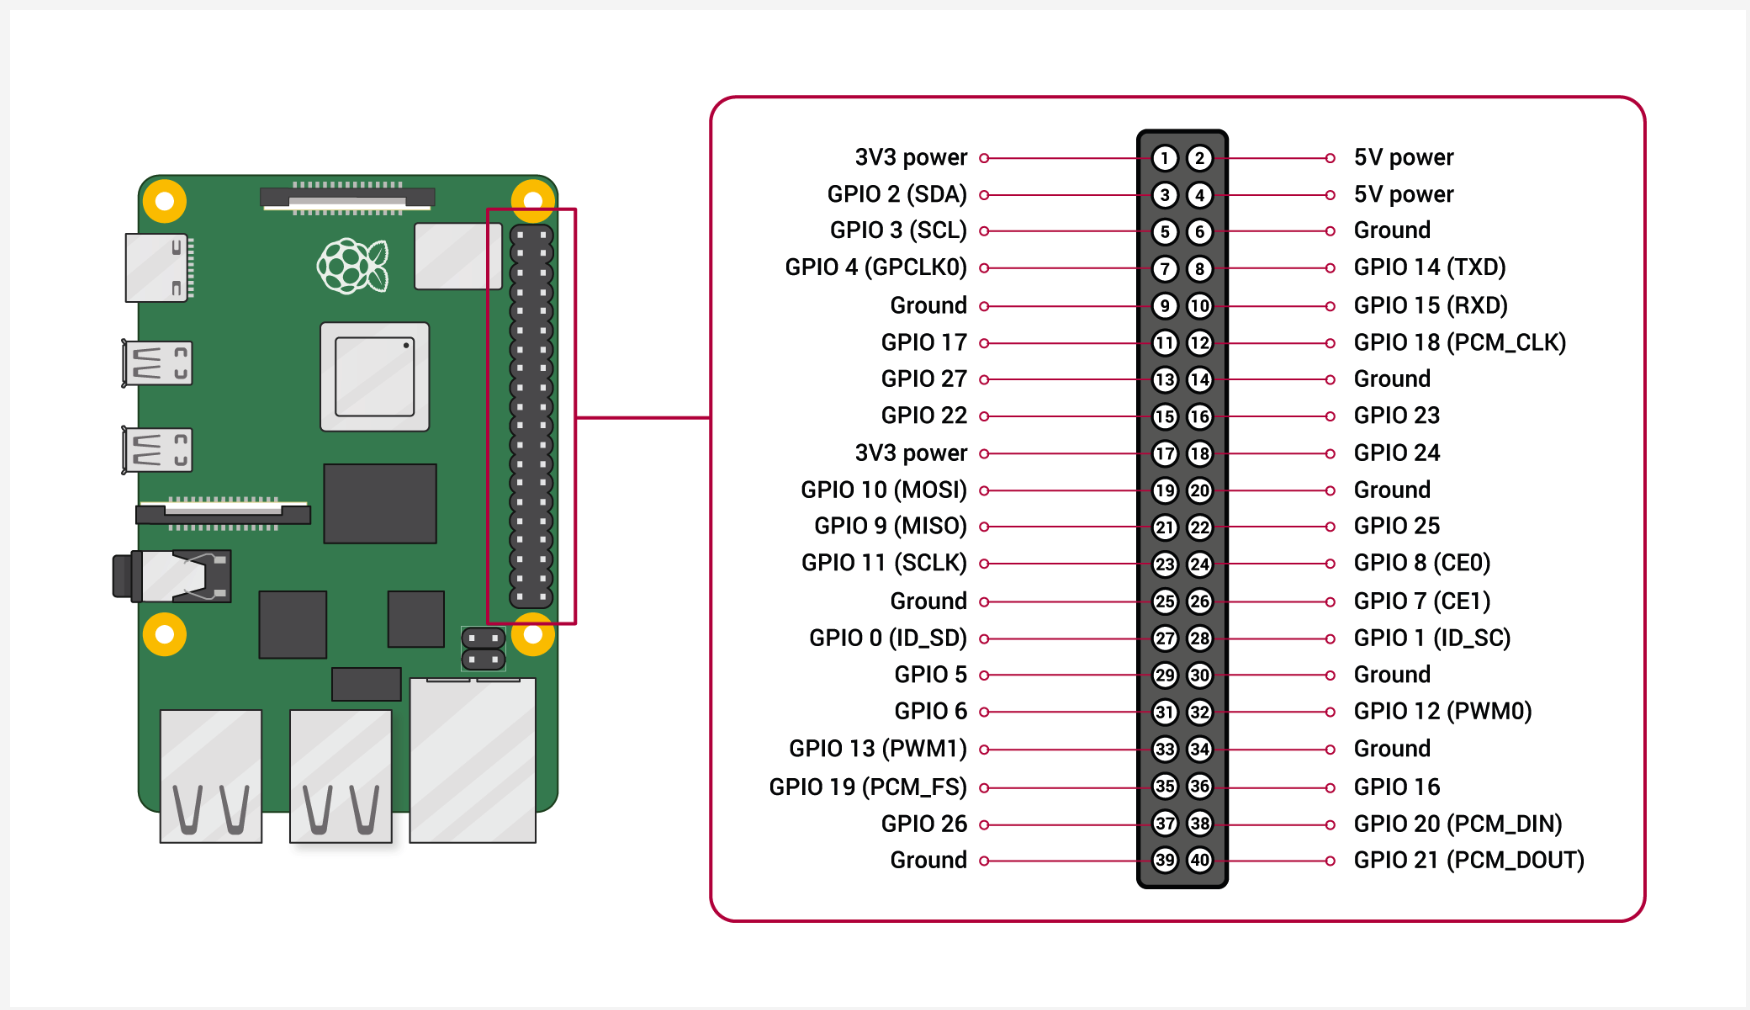
\includegraphics[scale = 0.4]{part/Proyecto_ejecutivo/memoria_constructiva/raspb/img/raspberry}
    \caption[Rasberry schema]{Raspberry schema \\Fuente: }\label{fig:raspberry pins}
\end{figure}

\begin{figure}[H]
    \centering
    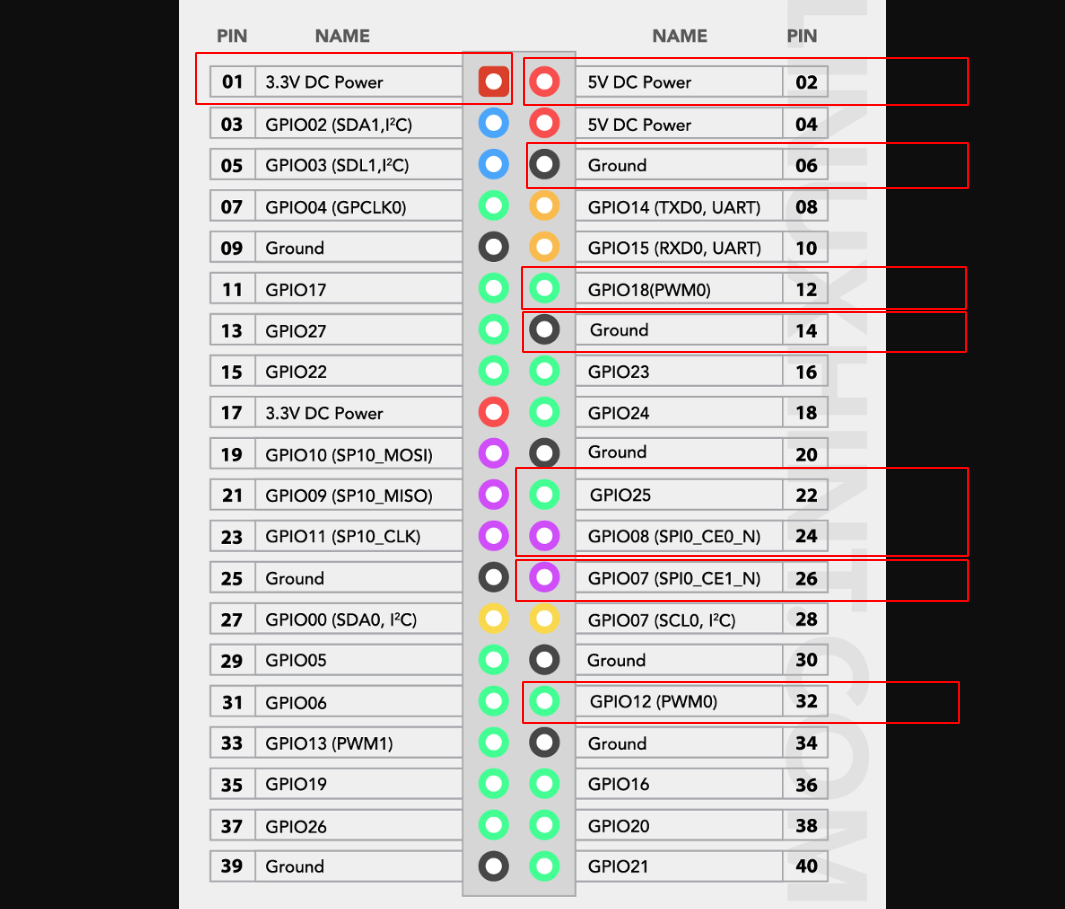
\includegraphics[scale = 0.4]{part/Proyecto_ejecutivo/memoria_constructiva/raspb/img/gpio-pinout-raspberry-pi-01-used}
    \caption[Motor EMG30]{Motor EMG30 \\Fuente: Documento de especificaciones técnicas.}\label{fig:Used Pins}
\end{figure}